% Minimal LaTeX file for apta specification: 
%   use Tikz graph syntax between the two parts. 
% >> part1 
\documentclass{standalone} 
\usepackage[T1]{fontenc} 
\usepackage[utf8]{inputenc} 
\usepackage{tikz} 
\usetikzlibrary{graphs,arrows,quotes,positioning} 
\standaloneconfig{margin=2em} 
\begin{document} 
\centering 
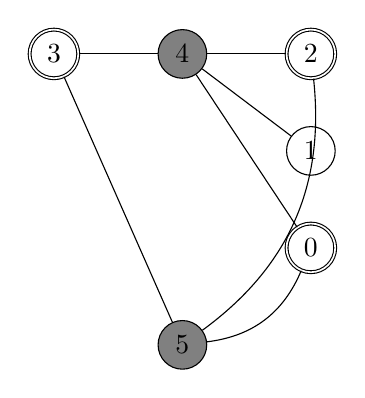
\begin{tikzpicture}[ 
			>=stealth', 
			accept/.style={double}, 
			reject/.style={fill=gray}, 
			backward/.style={bend right}, 
			self loop/.style={to path={ 
			.. controls +(70:1) and +(110:1) .. (\tikztotarget) \tikztonodes}} 
	] 
	\graph [ 
			grow right sep=1.0cm, 
			branch down sep=0.6cm, 
			nodes={draw,circle}, 
			edge quotes={font={\scriptsize}, inner sep=0.3ex, auto=right, pos=0.35} 
			]{ 
% >> end of part1 

		3 [accept] -- {
		4 [reject] -- {
		2 [accept] ,
		1 ,
		0 [accept] },
		5 [reject] },
		5 -- [clear >, backward] 2,
		5 -- [clear >, backward] 0
% >> part2 
	}; 
\end{tikzpicture} 
% >> end of part2 

\end{document}
